\documentclass[11pt]{article}
\usepackage[margin=1in,headheight=22pt]{geometry}
\usepackage{lmodern}
\usepackage{amsmath}
\usepackage{graphicx}
\usepackage{booktabs}
\usepackage{tikz}
\usetikzlibrary{arrows.meta,positioning,fit,calc}
\usepackage{hyperref}
\usepackage[numbers]{natbib}
\usepackage{xcolor}
\usepackage{titlesec}
\usepackage{fancyhdr}
\usepackage{colortbl}

% Style tokens mapped from .omp/skills/mkslides/references/resdir.pptx.
\definecolor{arcnavy}{HTML}{1F497D}
\definecolor{arcblue}{HTML}{4F81BD}
\definecolor{arcred}{HTML}{C0504D}
\definecolor{arcgreen}{HTML}{9BBB59}

\titleformat{\section}{\normalfont\Large\bfseries\color{arcnavy}}{\thesection}{1em}{}
\titleformat{\subsection}{\normalfont\large\bfseries\color{arcnavy}}{\thesubsection}{1em}{}

\pagestyle{fancy}
\fancyhf{}
\fancyhead[L]{\small ARCMiS}
\fancyhead[R]{\small\thepage}
\renewcommand{\headrulewidth}{0.4pt}
\renewcommand{\headrule}{\hbox to\headwidth{\color{arcblue}\leaders\hrule height \headrulewidth\hfill}}

\hypersetup{colorlinks=true, linkcolor=arcblue, urlcolor=arcblue, citecolor=arcblue}
\title{ARCMiS: Agentic Repository-Level Code Migration\\for Small Language Models}
\author{Duc-Hanh Dang \and Tu-Duc Nguyen\\
University of Engineering and Technology, Vietnam National University, Hanoi\\
\texttt{hanhdd@vnu.edu.vn}, \texttt{23021534@vnu.edu.vn}}
\date{October 2026}

\begin{document}
\maketitle

\begin{abstract}
We present ARCMiS (Agentic Repository-level Code Migration for SLMs), a
harness that migrates whole source codebases from one programming
language to another with small language models (SLMs, 27B parameters)
served locally on one consumer GPU. The harness is target-language
agnostic: each problem config names a source language, a target
language, and a build-plus-test command, so any legacy source can
target any language whose toolchain is expressible as such a command.
The current campaign instantiates this surface on C, Java, Go, and
Python sources with Rust targets, chosen for toolchain-scoring
determinism. The harness is a hierarchical multi-agent
system: a tier-1 orchestrator runs a ten-phase, evidence-gated state
machine and delegates over a task graph; a static three-tier tree puts
config-owned team leads (tier 2) over the specialist roles (tier 3), and
each lead runs its own inner loop from a scoped batch brief. A
deterministic guard hook inspects every tool call from every
tier, and an optional typed-decision judge arbitrates the ambiguous
remainder with deny-on-uncertain semantics. Role-agnostic hooks (trace,
continuation, per-role output budgets) live in a separate middleware
crate on the model-call path. All state lives on a
character-capped shared blackboard; snapcompact absorbs context overflow
by rendering discarded history to PNG bitmap frames instead of calling an
LLM summarizer. Scoring is toolchain-only: the configured build and test
commands must pass in the produced workspace, and agent self-reports
never gate. We report the state of an ongoing coverage-sweep campaign
over the 118-project ReCodeAgent corpus: as of 2026-10-06 the ledger
holds 55 round entries, 54 scored and 1 in flight, and 13 of the
campaign's 114-problem brief is
cleared (toolchain-verified compile and pass, each problem counted once
across retries). The cleared rate implies roughly $(114-13)/13 \times 10
\approx 78$ more campaign days at the current rate; we state it as an
estimate from the current rate, not a prediction. We also record the
binding constraints the campaign found: output-ceiling burn rate, the
Discovery context wall, engine-side transient failures, and set
selection. The results establish what a 27B local model can and cannot
do at repository scale, and no more.
\end{abstract}

\section{Introduction}
\label{sec:intro}

Repository-level code migration, translating an entire codebase from
one language to another while it keeps its behavior, is one of the
hardest
open tasks for coding agents. It needs three things at once: reading and
understanding code that does not fit in one context window, planning a
dependency-respecting translation order, and producing code that passes
real toolchains. Large frontier models can attempt this with ad-hoc
prompting. Small language models cannot. Small models are also the only
affordable option for sustained local use: they run on one consumer GPU,
cost nothing per token, and keep proprietary source on the machine.

ARCMiS targets exactly this regime. It migrates source codebases with a
27B model served locally on a single RTX~3090 (through the netmind
provider path against the local inference engine). The harness is
target-language agnostic: every problem config carries a source
language, a target language, and the test command that scores the
result, so the same orchestration, phase machine, and scoring rule apply
to any legacy source and any target expressible as a build-plus-test
command (Section~\ref{sec:targetlang}). The current campaign chose Rust
as its first target family for the coverage sweep; the dataset
families span C, Java, Go, and Python sources, and no non-Rust run has
been scored yet. The design
constraint that shapes the whole system is \emph{honesty of scoring}: an
agent's claim of success counts for nothing. A run succeeds only when the
configured target toolchain compiles the produced workspace and its test
command
exits zero. LLM-graded proxy scores, when recorded at all, never gate.

This paper makes four contributions:
\begin{itemize}
\item A hierarchical multi-agent methodology for repository-level
  migration with small models: a tier-1 orchestrator, a static
  config-owned tree of tier-2 team leads over ten tier-3 specialist
  roles, a ten-phase evidence-gated state machine, and a shared
  blackboard (Section~\ref{sec:method}).
\item A middleware separation: the role-agnostic model-call hooks
  (trace, continuation patch, per-role output budgets) live in their own
  crate under the criterion that a middleware hook never names a role or
  the orchestration domain; the guard hook stays with the delegation
  contract (Sections~\ref{sec:method} and~\ref{sec:infra}).
\item A benchmark record for the coverage-sweep campaign, updated
  2026-10-06: 55 round entries in the per-round ledger over the
  ReCodeAgent \texttt{tool\_projects} corpus, 13 of the campaign brief's
  114 problems cleared with toolchain-verified workspaces (each problem
  counted once across retries), and honest per-round verdicts including
  the rounds that never compiled
  (Section~\ref{sec:results}).
\item A failure taxonomy for SLM agents at this scale, distilled from the
  campaign: think-truncation at output ceilings, provider shape
  rejections, stagnation loops, and ceiling burns, with the limits they
  impose on generality claims (Section~\ref{sec:discussion}).
\end{itemize}

Figure~\ref{fig:arch} shows the system. One orchestrator runs the phase
machine. One guard hook sits on every tool call from every tier. Three
config-owned team leads sit over the ten specialists, who do the work on
a shared blackboard; a tier-1 delegation naming a lead hands the batch
to the lead's inner loop.

\begin{figure}[ht]
\centering
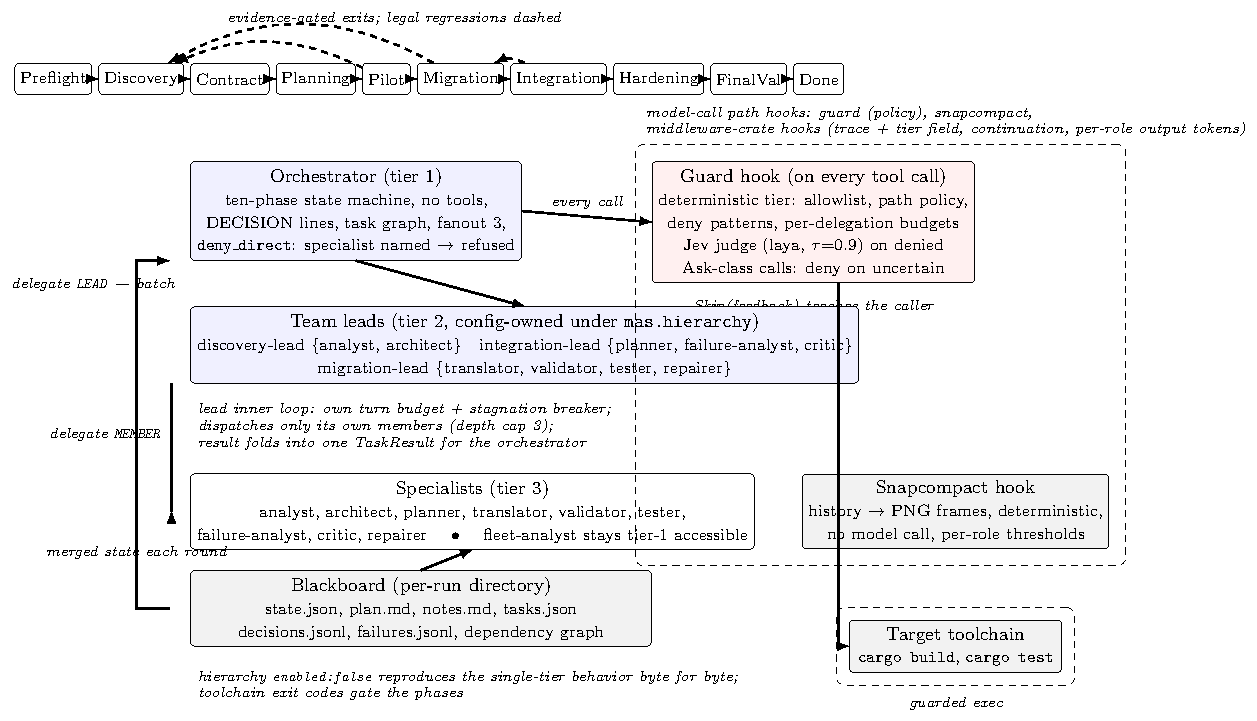
\includegraphics[width=\textwidth]{figures/fig1-architecture.pdf}
\caption{ARCMiS architecture. The tier-1 orchestrator rounds over the
ten-phase state machine and emits DECISION lines over a task graph. With
the hierarchy enabled, a delegation naming a specialist is refused
(\texttt{deny\_direct}) and the handoff form is a lead name; the lead
receives a scoped batch brief and runs its own inner loop over its
members (tier 3). The guard hook inspects every tool call from every
tier; denied Ask-class calls may arbitrate through the Jev judge (deny
on uncertain). The middleware crate holds the role-agnostic hooks
(trace, continuation, per-role output budgets); snapcompact attaches to
every role's call path. The configured target toolchain returns exit
codes to the
evaluator.}
\label{fig:arch}
\end{figure}

\section{Related Work}
\label{sec:related}

We group the related work into four categories: direct prior art on code
migration, multi-agent scaffolds that inspire this design, work that
justifies the methodology, and the pipeline agents we compare against.

\paragraph{Repository-level code migration.}
TransCoder~\cite{lachaux2020transcoder} translated functions between
C++, Java, and Python with unsupervised machine translation and evaluated
with unit tests. AlphaTrans~\cite{ibrahimzada2024alphatrans} is a
neuro-symbolic system that translates a whole repository and verifies
behavior with schemas and tests. AlphaTrans defines the repository-level,
behavior-verified translation problem that ARCMiS attacks with small
models instead of a neuro-symbolic pipeline.
CodaMosa~\cite{lemieux2023codamosa} escaped coverage plateaus
by mixing LLM test generation with search-based testing. Our
validator--tester loop applies that lesson with a per-module cap. Our
problem sets reuse the ReCodeAgent dataset's project pairs.

\paragraph{Multi-agent scaffolds.}
ReAct~\cite{yao2023react} interleaves reasoning traces with tool actions
and is the base loop of most single-agent migration scaffolds.
Reflexion~\cite{shinn2023reflexion}
adds verbal self-reflection across retries. Self-Refine~\cite{madaan2023selfrefine}
iterates a generate--feedback--revise loop. ARCMiS borrows the
iterate-on-failure shape but moves the feedback to deterministic judges
and toolchain evidence, because 27B models self-assess poorly. ReAct and
Reflexion define the reasoning-plus-action and
retry-with-feedback loops that every migration scaffold in this space
instantiates; ARCMiS keeps the loops but replaces model-graded feedback
with toolchain evidence. MetaGPT~\cite{hong2024metagpt} assigns a software company's
roles to LLM agents over standardized artifacts. AutoGen~\cite{wu2023autogen}
builds applications from conversing agents with human-in-the-loop
checkpoints. CAMEL~\cite{li2023camel} studies role-playing communicative
agents. MetaGPT, AutoGen, and CAMEL assume strong models and free-form
conversation; ARCMiS keeps the role decomposition but replaces
conversation with a parsed decision protocol, a static registry, and a
state machine, because conversation overhead is what small turn budgets
cannot afford. SWE-agent~\cite{yang2024sweagent} shows that a
well-designed agent--computer interface matters as much as the model;
that interface lesson is the basis for our hashline file tools and guard
hook. Agentless~\cite{xia2025agentless}
shows that a simple localizer--repairer--validator pipeline beats complex
agents on some tasks; the campaign's small-project verdicts agree in
spirit, since its two verified sets are the smallest C and Go sets.

\paragraph{Methodology justification.}
SWE-bench~\cite{jimenez2024swebench} anchored evaluation in executable
tests instead of model judgments, and we follow the same principle with
toolchain-only scoring: an agent pass counts only when the repository's
own tests pass. Meta-Harness~\cite{metaharness2026} evolves an executable harness
through an agentic outer loop where the proposer reads raw execution
traces from the filesystem; the campaign behind our benchmark
record follows that contract, with immutable per-run directories and
recorded lineage. Toolformer~\cite{schick2023toolformer} teaches
models to call APIs self-supervised. Gorilla~\cite{patil2024gorilla}
fine-tunes models for API invocation. ARCMiS uses neither: the 17-tool
surface is fixed, and the guard, not the model, enforces the calling
discipline, which a 27B model cannot learn reliably within its turn
budget. DeepSeek-R1~\cite{deepseek2025r1}
and Qwen3~\cite{qwen3_2025} make deliberate reasoning (\texttt{think}
blocks) standard on open models at our scale; those reasoning blocks
consume output-token budgets and drive the truncation failure mode in
Section~\ref{sec:discussion}. Speculative
decoding~\cite{leviathan2023speculative} makes local inference fast
enough for long agent runs, which is why the run budgets of this paper
fit on one GPU.

\paragraph{Hierarchical orchestration.}
Zhu et al.~\cite{zhu2026orchestration} survey multi-agent orchestration
frameworks and name hierarchical dynamic-adaptive orchestration as an
emerging pattern: static agents whose selection and composition at
runtime is dynamic, under multi-tier control. ARCMiS instantiates that
pattern in the small-model regime as a static three-tier tree: agents
are static (fixed registry, fixed preambles, fixed tool allowlists), the
lead-over-member assignments are config-owned, and the task graph, the
router chain, and the lead inner loops make selection dynamic. The
survey's deterministic-fallback and policy-enforcement guidance maps
one-to-one onto our guard hook and evidence-gated phases.

\paragraph{Pipeline agents for migration.}
ReCodeAgent~\cite{recodeagent2026} prescribes an
analyzer--planner--translator--validator pipeline for repository-level
translation and validation, and Ledger~\cite{ledger2026} prescribes a
manager--worker scaffold over a shared task ledger. Both exist as arXiv
preprints (arXiv:2604.07341, arXiv:2608.26480); we found no published
venue version, and our comparisons follow their prescribed algorithms
with that status unchanged. The ReCodeAgent paper's own comparison
set is Skel, Oxidizer, AlphaTrans, and SWE-agent, all re-run by its
authors with one frontier LLM (Claude 4.5 Sonnet) over 118 projects;
ARCMiS runs the same four problem-set families (crust, oxidizer,
alphatrans, skel) with a 27B local model, but the protocols differ on
model, scale, and scoring, so Section~\ref{sec:baseline} treats those
numbers as context, not a comparison.

\section{The ARCMiS Methodology}
\label{sec:method}

This section assumes no prior knowledge of the system. It defines the
vocabulary first, then the role taxonomy and its tiers, the
evidence-gated phase machine, the decision protocol with tiered
delegation, the blackboard, the guard, the budgets, the scoring rule,
and the per-problem language configuration that makes the harness
target-language agnostic.

\paragraph{Vocabulary.}
An \emph{orchestrator} is the single controlling agent of a run. It owns
the plan and the task list, and it never writes product code. A
\emph{specialist} is a role that does one kind of work (for example,
read the codebase, translate one batch, validate one batch, or repair
one diagnosed failure). A \emph{lead} is an intermediate agent that owns
a small team of specialists and runs an inner loop over them. A
\emph{delegation} is one unit of work handed from a controlling agent to
a lead or a specialist; the delegator writes a task text, and the
delegate works with its own tool access until it returns a result. A
\emph{round} is one turn of the orchestrator: it reads merged state from
the shared blackboard, emits one or more delegation decisions, and the
harness executes them before the next round. A \emph{phase} is one stage
of the migration pipeline, such as Discovery (read and map the source)
or Migration (translate every batch). A \emph{phase-exit evidence gate}
is a deterministic check that a phase's written exit condition holds
before the run may move forward; a gate rejection sends the orchestrator
back to work, and agent claims alone never pass a gate. A
\emph{stagnation breaker} is a deterministic stop rule: after a fixed
number of consecutive rounds with no completed task, the run ends with a
diagnosable artifact instead of looping. A \emph{ledger} is an
append-only record; the campaign keeps per-run ledgers of decisions and
failures inside each run directory, plus a per-round ledger
(\texttt{ROUNDS.yaml}) with one row per round and its verdict.

\subsection{Overview}

A run is one migration attempt against one problem: a source codebase
in language $L_s$ and a target language $L_t$, with a test command
defined
in the config (Section~\ref{sec:targetlang}). The harness (a Rust binary built on rig~0.42) spawns a MAS
whose members share one blackboard directory. Control is a static
three-tier tree: the orchestrator at tier 1 owns the plan and never
writes product code; team leads at tier 2 own one batch or phase slice
each; specialists at tier 3 own the work and never re-plan. What is
dynamic is selection and composition: the orchestrator may emit several
delegations in one round, the task-graph executor orders and gates them,
and a failing task can spawn a failure-analyst $\rightarrow$ repairer
sub-chain without any phase regression. Table~\ref{tab:roles} shows the
role taxonomy and the tier each role sits at.

\begin{table}[ht]
\centering
\begin{tabular}{llp{7.2cm}}
\toprule
Role & Tier & Responsibility \\
\midrule
Orchestrator & 1 & Owns plan and task list. Emits \texttt{DECISION} lines. No tools. \\
discovery-lead & 2 & Runs Discovery and Contract over \{analyst, architect\}. \\
migration-lead & 2 & Runs Planning, Pilot, and Migration over \{translator, validator, tester, repairer\}. \\
integration-lead & 2 & Runs Integration and Hardening over \{planner, failure-analyst, critic\}. \\
Analyst & 3 & Reads the codebase. Writes the source map and graphs. \\
Architect & 3 & Writes the migration contract (\texttt{analysis/brief.md}). \\
Planner & 3 & Produces dependency-ordered translation batches. \\
Translator & 3 & Writes target-language modules for one batch. \\
Validator & 3 & Judges one translated batch. Re-runs the suite. Read-only. \\
Tester & 3 & Adds tests. Runs the test command. \\
Failure-analyst & 3 & Classifies one failure into a five-category taxonomy. \\
Critic & 3 & Runs the end-of-run adversarial review. Read-only. \\
Repairer & 3 & Fixes one diagnosed failure. \\
Fleet-analyst & 1 & Model-ladder promotion advice; stays tier-1 accessible (no artifacts, no isolation value). \\
\bottomrule
\end{tabular}
\caption{The role taxonomy and tiers. Tier 1 is the orchestrator, tier 2
the team leads, tier 3 the specialists. The lead set is config-owned
(\texttt{mas.hierarchy}); with the hierarchy disabled the run is
byte-identical to the single-tier design. The \texttt{deny\_direct} gate
refuses a tier-1 delegation that names a specialist, so the handoff form
under hierarchy is the lead name. The preflight validator rejects a
member that sits in two teams and a lead without a prompt file.}
\label{tab:roles}
\end{table}

\subsection{Phase state machine}

The run walks ten phases: \textsf{Preflight}, \textsf{Discovery},
\textsf{Contract}, \textsf{Planning}, \textsf{Pilot}, \textsf{Migration},
\textsf{Integration}, \textsf{Hardening}, \textsf{FinalValidation},
\textsf{Done}. Forward transitions are earned. The orchestrator's
\texttt{done} verb is accepted only when the phase's exit condition holds
\emph{and} at least one delegation completed in the phase (the
\texttt{phase\_delegations} counter). Regressions are legal and recorded.
\textsf{Pilot} and \textsf{Migration} may fall back to \textsf{Discovery}
on a missing dependency, \textsf{Integration} to \textsf{Migration}, and
so on. Anything else is a programming error, not a model decision. Each
phase has a written exit condition in the orchestrator prompt. For example,
\textsf{Contract} requires \texttt{analysis/brief.md} to exist with a
validator pass covering it. \textsf{FinalValidation} requires the
configured toolchain command to exit zero on the target workspace.

\begin{table}[ht]
\centering
\begin{tabular}{llll}
\toprule
\# & Phase & Exit evidence & Legal regressions \\
\midrule
0 & Preflight & deterministic gates, no model call & --- \\
1 & Discovery & source map + brief cite every module & --- \\
2 & Contract & \texttt{brief.md} + validator pass & --- \\
3 & Planning & every module in one batch, order compiles & --- \\
4 & Pilot & one batch translated, verified, tested & Pilot$\to$Discovery \\
5 & Migration & every batch translated and verified & Migration$\to$Discovery \\
6 & Integration & full test suite green & Integration$\to$Migration \\
7 & Hardening & critic verdict is pass & Hardening$\to$Integration \\
8 & FinalValidation & toolchain rerun exits zero & FinalVal.$\to$Integration \\
9 & Done & --- & --- \\
\bottomrule
\end{tabular}
\caption{The phase state machine. Forward moves are evidence-gated.
Regressions are recorded, not hidden.}
\label{tab:phases}
\end{table}

The phase machine is also the campaign's diagnostic instrument. Every
stall in Section~\ref{sec:results} is reported as the phase where the run
stopped (\textsf{Discovery} or \textsf{Contract} for most failures), so a
reader can see at which capability boundary the harness, not the model,
gave up.

\subsection{Decision protocol and tiered delegation}

The orchestrator answers each round with plain text whose lines carry
\texttt{DECISION:} verbs: \texttt{delegate ROLE | TASK [|
  after:t2,t3]}, \texttt{replan}, \texttt{escalate},
\texttt{done}. Parsing text instead of expecting tool calls removes a
whole failure class of small-model agent runs: malformed tool-call JSON
that the inference server rejects with HTTP 500. The
orchestrator gets \emph{no tools at all}. The round prompt
carries the plan, notes, task list, ledger tail, and state, so the model
cannot spend turns re-reading files.

Each \texttt{delegate} decision becomes a task node with optional
\texttt{after:} dependencies (Figure~\ref{fig:delegation}). Direct tasks
run under the task-graph executor: the ready set (all dependencies done)
runs concurrently, one dispatch per job, joined in ready-set order so the
outcome stays deterministic (ADR 0029). A single dial, \texttt{fanout}
in the MAS config, bounds the tier-1 ready set and the lead's member
dispatches alike; its documented meaning is engine-instance
parallelism, and it carries no per-set value (no-tuning rule). The
outer-loop sweep driver sizes its own GPU-slot waves with a separate
\texttt{SLOTS} knob (Section~\ref{sec:sweep}). With the hierarchy enabled, the
\texttt{deny\_direct} gate refuses a delegation that names a team
specialist, and the handoff form is \texttt{delegate migration-lead |
  ...}: the tier-1 round prompt lists the lead names in ROLE. Routing is
a three-stage chain: the orchestrator's role hint, then a
deterministic keyword pass over the task text, then (as a last resort)
the router model. After each round the orchestrator re-scores the task
list and sees merged state, so a failing task can spawn a
failure-analyst $\rightarrow$ repairer sub-chain without any phase
regression.

\paragraph{The lead inner loop.}
A tier handoff is context management. The lead receives a scoped batch
brief (task text, the run contract, and the plan and notes tails under
the existing \texttt{plan\_cap}/\texttt{notes\_cap} caps), not the
orchestrator's history. Its inner loop parses every \texttt{DECISION:
  delegate MEMBER | task} line in the lead's answer, dispatches the
listed members concurrently through the same execution path as tier 1
(bounded by the same \texttt{fanout} dial; over-fanout dispatches are
deferred to the next round with a note in the transcript), and ends on
\texttt{done}, its own turn budget, its own stagnation breaker, or a
model failure. The lead dispatches only its own members (depth cap 3: lead names are not roles,
so a lead cannot dispatch another lead), and its result folds into one
\texttt{TaskResult} for the orchestrator. A cross-team or lead-named
dispatch draws a logged refusal and counts toward the stagnation
breaker. The lead's turn budget absorbs retry loops, which keeps batch
churn out of the tier-1 history.

\begin{figure}[ht]
\centering
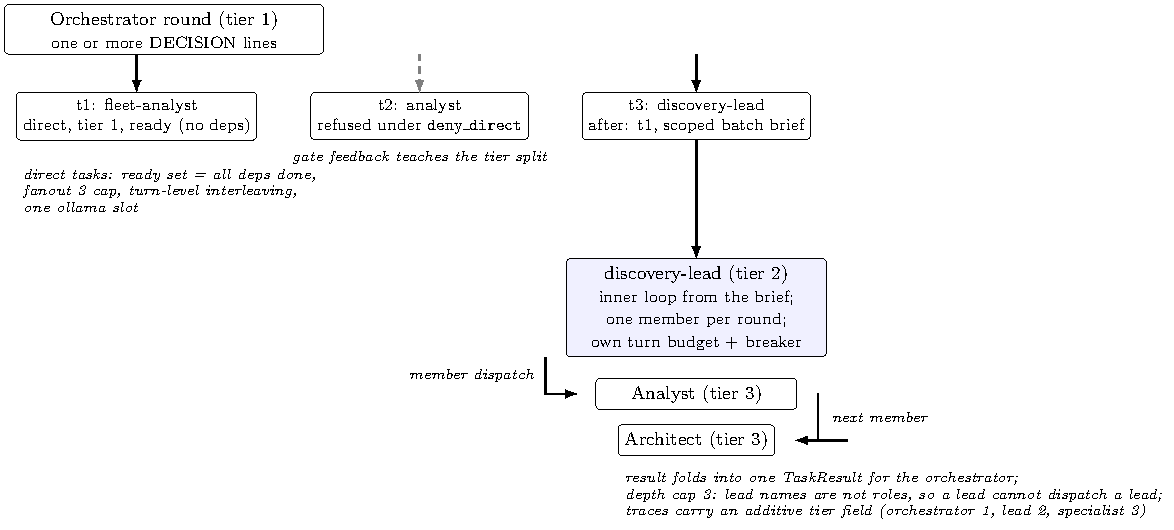
\includegraphics[width=0.92\textwidth]{figures/fig2-delegation.pdf}
\caption{Tiered delegation. The orchestrator (tier 1) emits DECISION
lines; the task graph executes the concurrent ready set of direct
tier-1 tasks whose dependencies
are done, bounded by the \texttt{fanout} dial. A delegation naming a lead hands the
batch to the lead's inner loop: the lead runs from a scoped batch brief,
dispatches its own members (tier 3) concurrently under the same dial,
and folds the result into one
TaskResult. Delegation events and traces carry an additive tier field
(orchestrator 1, lead 2, specialist 3).}
\label{fig:delegation}
\end{figure}

\subsection{Blackboard}

All mutable state lives in a per-run directory written by the blackboard
crate: \texttt{state.json} (phase, counters), \texttt{plan.md} and
\texttt{notes.md} (character-capped at 4000 and 8000), \texttt{tasks.json}
(task list mirror), \texttt{decisions.jsonl} and \texttt{failures.jsonl}
(ledgers), and a dependency graph. Character caps keep the shared state
inside one read for a 16k-token context window; the tuned config raises
the per-call window to 65536 with read gating (Section~\ref{sec:setup}),
and the caps still bound what the orchestrator prompt itself carries. The
writer truncates with an elision marker rather than silently growing the
context of every later reader.

\subsection{Guard hook and the Jev judge}

Every tool call from every agent at every tier passes one
\texttt{on\_tool\_call} hook. The deterministic tier of the guard (a
policy tier, not a hierarchy tier) inspects the role
allowlist (from static tool metadata), path policy (\texttt{source/} is
read-only, writes must stay inside the workspace), deny patterns for bash
(\texttt{rm -rf}, \texttt{git push}, package installs, network commands,
\texttt{sudo}), and per-delegation tool-call budgets. Rejections return
\texttt{Skip(feedback)}: the model sees the reason and adjusts the call,
and the breaker counts repeats. The guard lives in the orchestrator
crate, beside the delegation contract it enforces; the arbitration seam
below it is the only model-policed slot.

Calls that the deterministic tier marks ambiguous (Ask-class) fall to
an optional model-arbitra\-tion tier built on the laya typed-decision
crate,
following the Jev-as-a-judge pattern~\cite{li2026jevjudge}. The judge is
a small decision-only model that renders one typed \texttt{choice}
verdict per consultation in a single forward pass, with confidence $q$
defined as the maximum label probability. A confidence cascade with
$\tau = 0.9$ accepts confident verdicts; below $\tau$, on any load or
inference error, on foreign labels, or with the judge disabled, the
guard keeps its deterministic denial. The judge can only widen one
denial; it never bypasses a tier that passed the call, and budget
denials for non-ask tools are never arbitrable. Deny-on-uncertain is
the invariant: the escalation path is the existing deny, because with
one model in the loop there is no stronger judge to pay. The
deterministic rules stay above the judge: allowlist, path policy, and
budgets are untouched.

\subsection{Budgets, breaker, fleet ladder}

Budgets are per role class: orchestrator turns per round (20), worker
turns per delegation (40), judge turns (40, kept small in spirit by
prompting judges to promise few calls), lead turns per handoff
(\texttt{turns} per team in the hierarchy config; the smoke run's
migration-lead worked under a budget of 8), and a
run-level round ceiling. A deterministic stagnation breaker stops the run
after \texttt{stagnation\_rounds} (3) consecutive rounds with no completed
task, after repeated consecutive phase failures, or when a derived token
estimate exceeds the run ceiling; each lead carries its own breaker
under the same rule. It never consults a model. In the
campaign the breaker was the graceful exit: most stalled runs ended as
``3 consecutive rounds without a completed task,'' which is a diagnosable
artifact, not a hang. The fleet analyst owns a model ladder (weakest
first, config-driven) and promotes a role one rung on repeated failure.
Per-role output-token and think overrides are config knobs introduced
during the campaign (Section~\ref{sec:results}).

\subsection{Scoring}
\label{sec:scoring}

A run succeeds only when the evaluator reruns the target toolchain (the
build and test commands from the problem config) in the produced
workspace and every test passes. Agent self-reports are recorded but
never trusted. This rule exists because self-report traps are real:
an agent can write a passing per-problem record over an empty
workspace, and a status string carries no signal while an exit code
does. The scorer re-runs the
toolchain itself, and traces and score paths count tool-call activity, so
a healthy tool-only turn (empty text, real tool calls) is never misread
as a failure. Each scored round lands in one of five verdict classes:
\textsf{SOLVED} or \textsf{CLEARED} (the workspace compiles and its
suite passes), \textsf{VERIFIED-WORKSPACE} (the run stopped before
\textsf{done}, but the produced workspace scores green), \textsf{NOT
CLEARED} (the run closed without a green workspace), and
\textsf{ABORTED} (the run died before a close, typically on an
engine-side transient). The coverage scoreboard counts only
\textsf{SOLVED} and \textsf{CLEARED}.

\subsection{Target-language configuration}
\label{sec:targetlang}

The harness is target-language agnostic by construction. Each problem
config (rendered per round from \texttt{scripts/round-template.yml})
carries three language-facing keys: \texttt{source.language} names the
legacy language the translator reads, \texttt{target.language} names the
language it writes, and \texttt{target.test\_command} is the shell
command whose exit code and test counts score the run. The pipeline
(phases, roles, gates, breakers) never names a language; the agents read
the target language from the run metadata, and the run metadata also
carries the configured test command; the evaluator runs
whatever command the config carries. In principle any legacy source
language can target any language whose toolchain is expressible as a
build-plus-test command.

The current campaign instantiates this surface with Rust as the target
for every scored round: \texttt{target.language: rust} and a
\texttt{cargo test} command, chosen for toolchain-scoring determinism
(build and test exit codes, machine-parsable pass counts). The dataset
spans four source languages, C, Java, Go, and Python
(Table~\ref{tab:problems}), but no non-Rust run has been scored; the
generality claim rests on the configuration surface, not on scored
non-Rust runs. The scorer implementation
(\texttt{scripts/rescore.py}) now carries a language table: per-language
build commands (cargo, go, maven) with language-native test-count
parsers for cargo, pytest-style, go, and maven output, plus project-root
detection for all five targets (Rust, Go, Java, Python, JavaScript). The
scorer infers the target language from the detected manifest when the
config omits it, and the manifest and run metadata now carry the
configured \texttt{test\_command}. The validator and translator prompt
stubs list per-language stub markers, and the bench scorer fails loud
with an \emph{unsupported} status for unknown target languages. The
remaining Rust-only piece is the sweep template's target default
(\texttt{target.language: rust} in \texttt{scripts/round-template.yml},
with no target placeholder in the sweep driver); that is a config-layer
item queued for the next campaign boundary. No non-Rust round has been
scored, so generality rests on the config surface plus the now
language-neutral scorer, pending a scored non-Rust round;
Section~\ref{sec:limitations} records this.

\section{Supporting Infrastructure}
\label{sec:infra}

Five components carry the model-call path and the workspace boundary,
and one crate boundary keeps them honest. Each exists because a measured
failure mode demanded it, and each one is a hook or a pure tool layer,
outside agent code.

\paragraph{Middleware crate.}
The role-agnostic rig \texttt{AgentHook} implementations live in their
own crate, \texttt{ARCMiS/lib/middleware}: the trace hook (one trace
record per model call, tool call, and tool result, now carrying the
additive tier field), the continuation patch
(\texttt{TrailingUserMessageHook}), and the per-role output-token hook.
The split criterion is that a middleware hook never names a role, a
fleet, or the orchestration domain: it reads only hook event data plus
its own constructor parameters. Which hook runs for which role, with
which thresholds, is domain policy and stays in the agents crate. The
guard stays beside the delegation contract in the orchestrator crate,
because its allowlist and path policy are the delegation contract, not a
generic hook parameter.

\paragraph{Hashline file tools.}
File tools (\texttt{read}, \texttt{write}, \texttt{edit}) address content
through hashline tags (\texttt{PATH\#TAG}). Edits name the tag they
replace. A stale tag is an invalidation, not a silent overwrite. This
gives the guard a path-shaped argument to inspect and gives the model a
cheap merge-conflict signal.

\paragraph{Snapcompact.}
When the projected input of the next model call exceeds a per-role token
threshold, the snapcompact hook keeps the most recent messages verbatim.
It serializes the discarded history to dense text, renders that text to
PNG frames with a bundled public-domain 8x13 BDF bitmap font, and
attaches the frames as image blocks. The pass is deterministic (same
history in, same frames out) and costs no model call. LLM summarization
both spends budget and distorts. The hook lives in its own crate
(\texttt{snapcompact}); the per-role threshold wiring stays with the
registry, because threshold selection is domain policy. It attaches to
every role, with lower thresholds for the long-context specialists
(translator, validator) that need it most, and snapcompact events appear
in the traces, which makes context growth observable per agent.

\paragraph{Continuation patch.}
The Qwen chat template of the inference server rejects a message list
that ends
with tool results and carries no trailing user query (HTTP 500, ``no user
query found in messages''). rig 0.42 produces exactly that shape on every
multi-turn tool continuation. A completion-call hook appends a synthetic
user message (``Tool results above. Continue the task from here.'') to
the history. Without it, each rejected call burns a provider retry of
15--55~s.

\paragraph{Tool sandbox.}
Tool executions run against snapshot-gated workspaces, so the harness
can roll back a bad write without touching the source tree.

\section{Experimental Setup}
\label{sec:setup}

This section fixes the configuration that produced every number in
Section~\ref{sec:results}: the model and hardware, the four dataset
families, the budgets, the per-run protocol that the harness evolution loop
followed, and the coverage-sweep mechanics.

\paragraph{Model and hardware.}
All reported runs use a 27B reasoning model served locally on one
RTX~3090 through the \texttt{netmind} provider path. The current engine
is the local \texttt{ninfer} server serving \texttt{qwen3.8-27b}.
The
per-call configuration is
\texttt{num\_ctx} 65536 with guard read gating,
\texttt{max\_out\allowbreak{}put\_to\allowbreak{}kens} 8192 with
translator and architect raised
to 16384, temperature 0.2, \texttt{fanout} 2, and a 7200-second wrapper
timeout. Earlier configuration points are quoted in
Section~\ref{sec:results} only where the campaign refuted them.

\paragraph{Problem sets.}
The dataset is the ReCodeAgent \texttt{tool\_projects} directory,
organized in four source-language families: \texttt{alphatrans}
(Java, 4 problems),
\texttt{crust} (C, 100), \texttt{oxidizer} (Go, 7), and \texttt{skel}
(Python, 8), for
119 problem directories on disk in total. The campaign brief states 114
problems; the small gap comes from brief-time family bookkeeping, and we
report both numbers. The coverage sweep walks the families in
LoC-ascending order, one problem at a time, and counts a problem
\emph{cleared} when one scored round produces a workspace whose
configured toolchain compile and test commands both exit zero. In this
campaign every family targets Rust
(Section~\ref{sec:targetlang}). A problem cleared
once stays cleared; retries of a not-yet-cleared problem do not change
the count (Table~\ref{tab:verdicts}).

\begin{table}[ht]
\centering
\begin{tabular}{llrl}
\toprule
Family & Source language & Problems & Role in the sweep \\
\midrule
crust & C & 100 & main coverage walk \\
oxidizer & Go & 7 & coverage walk (paired slots) \\
skel & Python & 8 & coverage walk (source only, no bundled tests) \\
alphatrans & Java & 4 & coverage walk (largest sources) \\
\bottomrule
\end{tabular}
\caption{The ReCodeAgent \texttt{tool\_projects} dataset families, as
counted on disk, with the source language of each family. The sweep
walks problems in LoC-ascending order. In this campaign every family
targets Rust (the per-problem config fixes \texttt{target.language:
  rust} and a \texttt{cargo test} command,
Section~\ref{sec:targetlang}); the harness config surface supports other
targets, and no non-Rust round has been scored. The campaign
brief states 114 problems against 119 directories counted on disk; both
numbers are reported.}
\label{tab:problems}
\end{table}

\paragraph{Budgets.}
The MAS configs fix \texttt{max\_rounds} 20, orchestrator turns 20 per
round, worker turns 40 per delegation, judge turns 40, and the stagnation
breaker at 3 rounds. \texttt{plan\_cap} 4000 and \texttt{notes\_cap} 8000
bound the blackboard documents.

\paragraph{Protocol and campaign loop.}
One process per run, fresh workspace per run. Every run
leaves an immutable experiment directory: \texttt{manifest.json} (model,
budgets, git revision, parents, hypothesis), config,
\texttt{traces/turns.jsonl} (one line per model call, tool call, and tool
result), the produced \texttt{workspace/}, captured streams, and a
\texttt{result/} aggregate with a staged failure taxonomy
(\texttt{setup}, \texttt{analyze}, \texttt{plan}, \texttt{translate},
\texttt{verify}, \texttt{evaluate}). Scoring is toolchain-only
(Section~\ref{sec:method}). The harness evolution loop over these runs kept
the problem set and evaluator fixed; every change
was harness-side. Section~\ref{sec:optmethod} states the loop's
contract and the per-iteration hypotheses.

\subsection{Coverage-sweep mechanics}
\label{sec:sweep}

The current execution mode is a parallel coverage sweep over the
dataset. The outer-loop
driver \texttt{scripts/sweep.sh} reads a pair file of problem paths,
sizes each wave with a \texttt{SLOTS} knob (GPU inference slots,
staggered), and launches one immutable experiment directory per round.
A coverage round targets one untouched problem; a \texttt{NOT CLEARED}
problem may retry, and the scoreboard counts the problem once, cleared
only when a round passes. The in-harness parallelism (ADR 0029) is
separate: the \texttt{mas.fanout} dial bounds concurrent dispatches
inside a run, while \texttt{SLOTS} bounds concurrent runs. Wave 1 of
the current arm (\texttt{PAIRS-ninfer-w1.txt}) carries 18 problems,
launched over two GPU slots with staggered starts.

\paragraph{Round naming.}
Rounds carry a global counter in their ledger tags. A wave that
reuses a slot number collides with a historical row; the ledger keeps
both, and the later row takes an \texttt{.r2} suffix with a distinct
\texttt{candidate\_id}. So one problem can span several rounds
(retries), and no round is silently dropped. Since commit
\texttt{e62c2f6} the driver numbers all new launches from a global
counter, so tag collisions occur only on
the pre-fix rows.

\paragraph{Wave state at build time.}
The sweep runs in waves of paired GPU slots. Wave 1 (18 problems) and
wave 2 (17 problems) closed on 2026-10-04 and 2026-10-05: one
\textsf{NOT CLEARED} close in wave 1 (heapq) and three in wave 2 (fft,
bst, remimu). Wave 3 carries 17 problems: rbt closed \textsf{NOT
CLEARED} on 2026-10-06, and skp remains in flight at build time, so no
verdict from that round appears in the results. Both closed waves
recorded repeated engine-side admission-503 deaths and in-place
launcher restarts inside one experiment directory, which matters for
wall-clock accounting (Section~\ref{sec:honestwalls}).

\subsection{Harness evolution methodology}
\label{sec:optmethod}

The campaign follows a Meta-Harness-style harness evolution loop
\cite{metaharness2026}: an agentic outer loop whose proposer reads the
full experiment history from the filesystem and proposes the next
harness change. The loop runs under five contract rules, each enforced
by the experiment tree rather than by trust:

\begin{itemize}
\item \textbf{Immutable per-candidate directories.} One experiment per
directory under a dedicated artifacts root. The directory is immutable
after the run: the proposer reads, never writes. It carries
\texttt{manifest.json}, the produced workspace, raw traces (one JSON
line per model call, tool call, and tool result), and the scored
result.
\item \textbf{Pre-registered causal hypothesis.} Each manifest records
a one-sentence hypothesis before launch, plus \texttt{parents} links to
prior experiment ids. Lineage lives in the manifests; search scripts
never reconstruct it. The proposer must name the mechanism its change
targets, so every refuted candidate stays attributable.
\item \textbf{Toolchain-only rescoring.} The scorer reruns the target
build and test commands inside the produced workspace; agent
self-reports never gate. \texttt{success: true} requires translation to
complete and the toolchain test command to exit zero.
\item \textbf{Pareto frontier.} \texttt{frontier.py} reads only the
experiment tree and orders candidates by verified pass, per-problem
test count, and wall time. A candidate dominates another when it is
not worse on every key and strictly better on one. The frontier, not
any single score, selects the champion.
\item \textbf{Converge-or-rotate.} The 3-cycle rule: if the best
candidate on a set shows no frontier gain across three consecutive
cycles, the set has converged. A converged champion either closes the
loop or rotates to fresh, unseen sets under the exact tuned defaults
as an out-of-sample check.
\item \textbf{No-tuning rule.} The problem set and the evaluator stayed
fixed throughout; every change was harness-side. No run
config was edited per set, and no prompt was tuned against a known
failure.
\end{itemize}

The loop found every binding constraint by reading raw traces, not
summaries. Table~\ref{tab:lineage} attributes each lineage step to its
recorded hypothesis; Figure~\ref{fig:lineage} plots the verified-test
lineage it produced.

\begin{table}[ht]
\centering
\begin{tabular}{@{}p{1.1cm}p{5.2cm}p{7.6cm}@{}}
\toprule
Cycle & Hypothesis (from the manifest) & Outcome \\
\midrule
c1 & think-only turns truncate at exactly the 4096-token output cap
(\texttt{finish\_reason=Length}, empty text); raise
\texttt{max\_output\_tokens} to 8192 & First verified migration:
nandc workspace passes 2 tests. Diagnosis came from raw traces, where
every dead delegation died at exactly the cap. \\
c3 & 31 of 41 stalled turns sat at the 16384 \texttt{num\_ctx} wall;
double context, add tool-aware traces for triage & Discovery
saturation fixed; nandc reaches 17 verified tests. \\
c10b & checkdigit's architect died at exactly 8192 output tokens;
raise the architect's per-role output cap to 16384 & Architect passes
Contract on the first try; 48-test champion. \\
c11b & identical-config rerun under a doubled 7200\,s wrapper timeout;
a completed 13/13 would be the first & 36 tests; killed by the
timeout ~6\,min after its last pass. \\
c12 & all-roles 16384 output override & \textbf{Refuted}: bigger burns
cost 10--20\,min per retry against 1--2\,min at 8192; total wrapper
throughput, not per-turn survival, is the metric. \\
c13 & revert to the translator-only 16384 override; reproduce or beat
c11b's depth & No depth gain; plateau closes the loop. \\
c14 & two fresh sets under the exact tuned defaults, no per-set
tuning & Both stall before Contract; out-of-sample generality not
established. \\
\bottomrule
\end{tabular}
\caption{Lineage steps and the pre-registered hypotheses that caused
them, quoted from the per-run manifests. The loop, not the prompt,
found each binding constraint: output-cap truncation (c1), the context
wall (c3), per-role output budgets (c10b), and the ceiling-throughput
trade (c12--c13).}
\label{tab:lineage}
\end{table}

\section{Results}
\label{sec:results}

The live record is the coverage-sweep campaign state as of 2026-10-06,
read from the per-round ledger (\texttt{ROUNDS.yaml}) and the experiment
tree. The ledger holds 55 round entries, of which 54 are scored and 1 is
in flight (skp, wave 3). The
problem set and evaluator never changed; every iteration changed the
harness. Every data path in this section reads from the per-run
artifacts. Table~\ref{tab:verdicts} gives the live scoreboard, and
Figure~\ref{fig:persets} shows the cleared problems per family.

\begin{table}[ht]
\centering
\begin{tabular}{@{}lrl@{}}
\toprule
Measure & Value & Source \\
\midrule
Dataset (counted on disk) & 119 problems & \texttt{tool\_projects} subdirectories \\
Dataset (campaign brief) & 114 problems & campaign brief \\
Rounds in ledger & 55 & \texttt{ROUNDS.yaml} (54 scored, 1 in flight) \\
\cellcolor{arcgreen}Unique problems cleared & \cellcolor{arcgreen}13 & SOLVED/CLEARED verdicts, counted once \\
In flight & 1 round (skp, wave 3) & not counted as a verdict \\
\bottomrule
\end{tabular}
\caption{Live campaign scoreboard at build time (2026-10-06). A problem
counts once even when several rounds cleared it (retries and
replicates).}
\label{tab:verdicts}
\end{table}

The 13 cleared problems are: leftpad, amp, ulidgen, gonameparts,
avalanche, colorsys, morton, libqueue, murmurhash, geofence, gfc,
2dpartint, and bhshell. The verdict mix over the 54 scored rounds is
19 SOLVED, 21 NOT CLEARED, and 14 ABORTED; one further entry
(IN FLIGHT, wave-3 skp) carries no verdict yet and is excluded from
every count. A problem may take
several rounds before one passes, so the round count exceeds the
problem count.

\begin{figure}[ht]
\centering
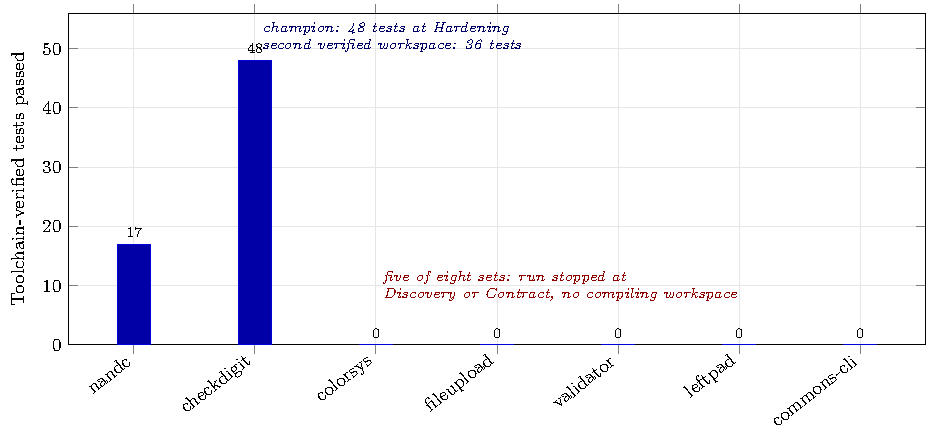
\includegraphics[width=0.94\textwidth]{figures/fig3-per-set.pdf}
\caption{Cleared problems per dataset family at the 2026-10-06
scoreboard (13 of the brief's 114). The figure preserves the earlier
four-day search campaign's per-set test peaks (nandc 17, checkdigit 48
and 36); the sweep-phase cleared problems are counted once per problem,
across retries, from the per-round ledger.}
\label{fig:persets}
\end{figure}

\subsection{Campaign rate and estimated time to complete}
\label{sec:rate}

The campaign opened on 2026-09-26 and has run through 2026-10-06: 10
campaign days. With 13 unique problems cleared, the observed rate is
1.3 problems per day. The dataset holds 114 problems per the
campaign brief (119 counted on disk), so the remaining work at the
current rate is about $(114-13)/1.3 \approx 78$ days. This is an
\emph{estimate from the current rate}, not a prediction: the LoC walk
ascends into larger problems, the
parallel arm (Section~\ref{sec:sweep}) raises throughput, and
engine-side transient failures dominate the
ABORTED class, so the rate will move in both directions. For scale, the
serial-era solved rounds (one problem at a time) took a median of
145 minutes of wall clock (15 solved rounds, ninfer era); the
wave-closed failed rounds run longer and carry restart overhead
(Section~\ref{sec:honestwalls}).

\subsection{Honest wall-clock accounting for failed rounds}
\label{sec:honestwalls}

The ledger \texttt{wall\_seconds} value covers only the final harness
segment of a round, because the launcher restarts the harness in place
after an engine-side admission failure. For the three wave-2 closes the
full-window walls are materially larger than the ledger values, and we
report both (Table~\ref{tab:honestwalls}). The rescore covers the final
segment only; the accounting note is part of the round record, not a
correction to it.

\begin{table}[ht]
\centering
\begin{tabular}{@{}llrr@{}}
\toprule
Round & Verdict & Ledger wall (s) & Full-window wall (s) \\
\midrule
fft (wave 2) & \cellcolor{arcred}NOT CLEARED & 76 & 2131 \\
bst (wave 2) & \cellcolor{arcred}NOT CLEARED & 1277 & 7962 \\
remimu (wave 2) & \cellcolor{arcred}NOT CLEARED & 50354 & 53084 \\
\bottomrule
\end{tabular}
\caption{Failed-round walls: the ledger value (final harness segment,
in-place restart accounting) against the full window from the first
trace to the close event. The ledger value is what the rescore covered;
the full-window value is what the campaign actually spent.}
\label{tab:honestwalls}
\end{table}

\subsection{Champion and lineage (earlier search campaign)}

The subsections that follow preserve the earlier four-day search
campaign's record (closed 2026-09-29), which the coverage sweep
superseded as the campaign's execution mode; they stay because the
lineage is where the harness's durable findings were established. The
champion run is the checkdigit candidate closed at
\textsf{Hardening} on 2026-09-28: 13 rounds, 14 delegations, 12 of 13
tasks done, and a translated Rust crate whose \texttt{cargo build} is
clean and whose test suite passes, toolchain-verified
in the produced workspace (12 \texttt{cargo test} cases including unit,
integration, and doc tests; the campaign scorer's rescore counts 48
test cases). The run stopped on the wrapper's runtime
timeout mid-\textsf{Hardening} after a repairer pass, not on a model
failure. Figure~\ref{fig:lineage} shows the lineage: the campaign peak is
two toolchain-verified oxidizer workspaces (48 and 36 tests on two
checkdigit candidates) and one nandc lineage carrying five generations.

\begin{figure}[ht]
\centering
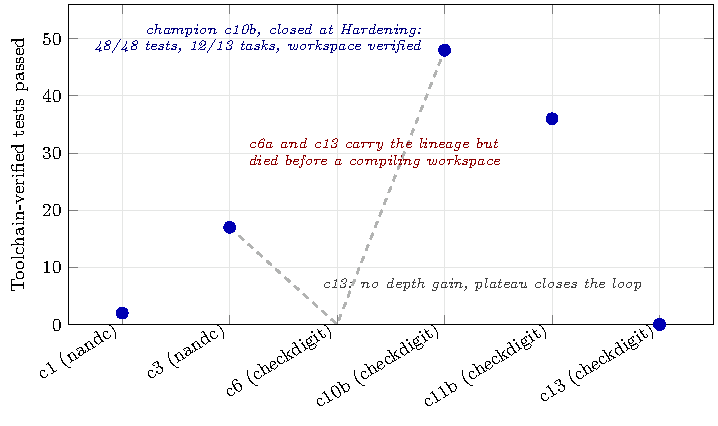
\includegraphics[width=0.9\textwidth]{figures/fig4-frontier.pdf}
\caption{Champion lineage by toolchain-verified tests passed, one point
per accepted hypothesis in the harness evolution loop. The nandc lineage
runs from the first verified migration (2 tests at Hardening, after the
c1 output-cap fix) to its 17-test generation (c3, after the context
raise). The checkdigit lineage peaks at 48 tests (c10b, after the
per-role output-cap raise), regresses to 36 (c11b, a favorable sample
rather than a config effect), and shows no depth gain at c13, whose
plateau closed the loop. Every binding constraint on this path was
found by the loop reading raw traces, not by prompt changes.}
\label{fig:lineage}
\end{figure}

The lineage records what each pre-registered hypothesis bought
(Table~\ref{tab:lineage}). The seed configuration plus trace hooks
produced the first verified workspace (2 tests) once the c1 hypothesis
removed the 4096-token think-truncation. The c3 read-scoping and
context-raise hypothesis fixed Discovery saturation on multi-file sets
and made the stall breaker the graceful exit (17 tests). The c10b
per-role output-cap hypothesis carried the architect past Contract,
which landed the 48-test champion. The c11b rerun under a doubled
timeout looked like progress at 36 tests but was a favorable sample,
and the regression test against it failed: the c12 all-roles 16384
override showed that bigger burns cost 10--20 minutes per retry against
1--2 minutes at 8192, and total throughput fell. The c13 revert to the
translator-only override showed no depth gain, and the plateau closed
the loop under the 3-cycle rule. The c14 rotation hypothesis then
failed out of sample: two fresh sets under the exact tuned defaults
stalled before Contract.

\subsection{Hierarchy validation (earlier campaign)}

Before the sweep phase opened, one smoke run validated the three-tier
hierarchy (Section~\ref{sec:method}) end to end on the GildedRose
set (a C source migrated to Rust), with the campaign champion as its
parent. The run
reached \textsf{Migration} in 13 rounds with 5 of 8 tasks done and a
green toolchain: the produced workspace's \texttt{cargo build} and
\texttt{cargo test} exit zero, and the \texttt{text\_test} binary
reproduces the source's 31-day walkthrough (day 0 through day 30)
line for line. The run is explicitly incomplete
(\texttt{completed: false}); it stopped on the stagnation breaker
after the migration lead exhausted its turn budget of 8 on verbose
task text. The delegation record shows the mechanics working as
designed: 7 tier-2 handoffs under the three leads, 19 lead turns, and
14 tier-3 member dispatches, with \texttt{discovery-lead} and
\texttt{migration-lead} trace records carrying the tier field
(tier 2) and their specialists tier 3. This is a validation of the
hierarchy mechanics, not a completed migration, and it does not change
the campaign verdicts.

\subsection{Campaign observations}
\label{sec:observations}

The wave-2 and wave-3 closes left a census of operational pathologies.
We record them as observations with evidence pointers; the root causes
are hypotheses under harness review, not confirmed defects.

\paragraph{Admission-503 census.}
Engine-side HTTP 503 admission and queue timeouts recur under
concurrent GPU-slot launches. A launcher retry re-enters the same
experiment directory in place, so one ledger round can span several
harness runs (two for fft, three for bst, three for remimu). The in-run
census for the wave-3 rbt close records 9 admission-503 deaths, 1
MaxTurns death at 40 turns, 2 output-cap (Length) deaths, and 1 gate
refusal. The harness carries admission backoff (max retries 4) and a
transient-stalled-round reprieve; the census is evidence that engine
capacity, not harness logic, dominated the failed closes.

\paragraph{MaxTurns grind pathology.}
Long grind rounds die at the worker turn ceiling. The remimu close is
the clearest case: 39.3M input tokens over the run, 30.4\% of output
burned as think blocks on think-enabled roles, 41 of 46 lead rounds
carrying a single dispatch, and 30 MaxTurns deaths across the wave-2
closes. The pattern suggests that a lead round which dispatches only one
member spends its round budget on sequencing rather than work, and that
think-enabled roles pay a large think share of the output budget. Both
mechanisms are measurable in the traces; both are candidates for the
next harness cycle, and neither is confirmed as the binding cause.

\paragraph{Gate and launcher semantics.}
Three observations name harness seams. First, delegations twice named a
\texttt{fleet-analyst} role that the dispatch grammar does not define;
the deny-direct gate did not block the unknown role, and the role lacked
a think override, so its output burned on think with empty text. The
dispatch-grammar reading is a question for an ADR-level review, not a
confirmed defect. Second, one gate rejected a \texttt{done} claim with
``no completed delegation'' and then accepted an identical claim with no
new delegations in between; the gate is not idempotent across identical
claims. Third, the sweep launcher treats exit code 0 as success, and a
stagnation-breaker exit is also 0, so a completed-but-failed run looks
successful to the retry loop. Each observation points at code whose fix
is mechanical; none is yet fixed, and none changes the verdicts.

\subsection{Capability boundaries}

The verdicts split the corpus into regimes, and the boundary tracks
corpus type and size, not LOC alone. The sweep-phase cleared problems
(13) are small C, Go, and Python sources, mostly under 400 source LOC;
the colorsys clearance showed the first Python-source set clearing with
a synthesized test suite (the \texttt{skel} family ships source only).
The alphatrans sets (Java, 8.6k--36k LOC) remain the hard regime:
commons-csv, the largest source ever attempted (about 11M tokens of
source), never cleared on coverage, but it reached \textsf{Planning}
with a translated crate that compiles and passes its 5 collected tests,
the deepest Java run on record, which showed per-module dispatch
keeps translator inputs inside the context window and the residual
constraint is wall time. The earlier campaign's c14 rotation evidence
(leftpad and commons-cli stalled under the then-tuned defaults) is
superseded: leftpad is now cleared, which shows the stall was a harness
defect the campaign later fixed, not a capability wall.

The binding constraints the campaign named are three. First, the
model's round-budget burn rate: ceiling burns plus slow artifact turns;
no ceiling policy, timeout raise, or context raise moved it. Second,
engine-side transients: the ABORTED class (14 of 54 scored rounds) is dominated
by engine 503 admission/queue-timeout deaths and one endpoint
migration; the harness now carries admission backoff and a
transient-stalled-round reprieve. Third, set selection: the LoC walk
skips nothing, so the harness meets every corpus type eventually; the
open question is the Java alphatrans regime, where no coverage
clearance exists yet.

\subsection{Baseline comparison: published context (different protocol)}
\label{sec:baseline}

One comparison surface exists in this paper: the published ReCodeAgent
record. \textbf{Label: different protocol.} ARCMiS never ran Skel,
Oxidizer, AlphaTrans, or SWE-agent on shared instances under one
protocol, so every cross-paper juxtaposition below is directional
context, not a comparison and not statistical.

\paragraph{Published ReCodeAgent numbers as context.}
The ReCodeAgent paper (arXiv:2604.07341, accepted at ASE 2026)
benchmarks ReCodeAgent against four techniques, reproduced by its
authors with the same LLM: Skel, Oxidizer, AlphaTrans, and SWE-agent,
over 118 real-world projects across four PL pairs (C$\to$Rust,
Go$\to$Rust, Java$\to$Python, Python$\to$JavaScript), all driven by
Claude 4.5 Sonnet with a 5{,}000-second per-agent budget. Its headline
results: 99.4\% compilation success; 86.5\% test pass rate over
validated developer tests against 25.7\% for the competing techniques
(2{,}107 validated tests total; per-technique TPR: Oxidizer 67.2\%,
Skel 93.2\%, AlphaTrans 188 of 1{,}181 executed tests, SWE-agent
78.3\% on the Crust subset); and 98.1\% on translated developer tests.
Table~\ref{tab:published} collects these published numbers.

\begin{table}[ht]
\centering
\begin{tabular}{@{}lll@{}}
\toprule
Technique & Published result & Protocol \\
\midrule
ReCodeAgent & 99.4\% CS, 86.5\% TPR & Claude 4.5 Sonnet, 118 projects \\
Skel & 93.2\% TPR (its benchmark) & reproduced with the same LLM \\
Oxidizer & 67.2\% TPR (its benchmark) & reproduced with the same LLM \\
AlphaTrans & 188/1{,}181 tests passed & reproduced with the same LLM \\
SWE-agent & 78.3\% TPR (Crust subset) & reproduced with the same LLM \\
\midrule
\multicolumn{3}{@{}l@{}}{Target language: ReCodeAgent scores mixed targets}\\
\multicolumn{3}{@{}l@{}}{(Rust, Python, JavaScript per pair); every scored}\\
\multicolumn{3}{@{}l@{}}{ARCMiS round targets Rust (Section~\ref{sec:targetlang}).}\\
\bottomrule
\end{tabular}
\caption{Published ReCodeAgent-record numbers
\cite{recodeagent2026}. These are the paper's own protocol: its
projects, its validated developer suites, its frontier model, and its
mixed target languages. ARCMiS
never ran Skel, Oxidizer, AlphaTrans, or SWE-agent on shared instances
under its protocol, and every scored ARCMiS round targets Rust, so this
table is context, not a comparison, and no
cross-paper statistical comparison with any ARCMiS number is valid.}
\label{tab:published}
\end{table}

Three protocol differences make these numbers non-comparable to every
ARCMiS number in this paper. First, the model: a frontier proprietary
model against one 27B quantized model on one GPU. Second, scale:
projects averaging 1{,}975 LOC (up to about 38{,}000) against our
82 to 36{,}356, with per-agent budgets of 5{,}000 seconds and an
average cost of \$15.3 per project. Third, validation: ReCodeAgent
translates and generates tests in both source and target languages and
uses author-validated suites withheld until after the run, whereas a
campaign pass requires the pre-registered evaluator commands to exit
zero on the produced workspace only. The sets overlap in family
(oxidizer, alphatrans, skel, crust), not in instance lists or scoring.
We therefore draw no ranking from the juxtaposition. What the comparison
does support is directional: the published record shows a multi-agent
pipeline with iterative validation outperforming single-shot and
neuro-symbolic baselines by wide margins on the same projects, which is
consistent with our finding that harness discipline, not model
prompting, carries small models past single-agent limits.

\section{Discussion}
\label{sec:discussion}

The campaign's value beyond the verdicts is the failure record. This
section names the four mechanisms that dominate it, the limitations that
bound every claim, and the threats to how the numbers were read.

\paragraph{Failure taxonomy.}
Four failure modes dominate the campaign record, and each one names the
harness change that addressed it.
(1)~\emph{Think-truncation}: with \texttt{think:true}, reasoning blocks
consume the output budget; a turn that dies at exactly the ceiling with
empty text and no tool call is a hard completion error, and retries
reproduce it deterministically at temperature 0.2. The architect and
planner burns at exactly 8192 tokens killed more runs than any other
mechanism; per-role output overrides address it.
(2)~\emph{Provider shape rejections}: the inference server's chat
template rejects message lists without a trailing user query, on tool
continuations
(patched by the hook, Section~\ref{sec:infra}) and on a first-call
request shape with an empty prompt field. A separate engine-side class
dominates the ABORTED verdicts: HTTP 503 admission and queue-timeout
deaths under concurrent slot bursts; admission backoff and a
transient-stalled-round reprieve address it.
(3)~\emph{Stagnation}: without a breaker, the orchestrator retries the
same delegation shape indefinitely. The 3-round breaker converts an
unbounded loop into the campaign's most common stop reason and its
graceful exit.
(4)~\emph{Ceiling burns}: an output ceiling kills a role only when the
whole artifact cannot fit, but the retry cost depends on where the
ceiling sits: 1--2 minutes at 8192, 10--20 at 16384. Total wrapper
throughput, not per-turn survival, is the metric, which is why a
translator-only override dominates an all-roles override, and why the
all-roles policy was refuted as a global default.

\paragraph{Limitations.}
\label{sec:limitations}
Four limits bound every claim in this paper. First, coverage, not
depth: the sweep counts a problem cleared when one round's workspace
passes the toolchain; it does not yet measure translation quality
against the source behavior, so the 13-cleared scoreboard is a
coverage rate, not a correctness rate. Second, target-language
generality: the design is target-language agnostic
(Section~\ref{sec:targetlang}), but every scored round targets Rust. The language-generality audit has closed, and its confirmed items are
fixed in the working tree: the scorer now has a language table, project
markers, and target-language inference; the validator hint is
language-neutral; the run contract carries \texttt{test\_command}; the
prompt stub markers are per-language; the bench scorer fails loud on
unknown languages. The sweep template's Rust default remains and is
queued for the next campaign boundary. No non-Rust round has scored
green yet, so the
generality claim rests on the configuration surface, not on results.
Third, the alphatrans (Java) regime: no Java set has cleared, so
generality across corpus types is
open, and any new harness idea must first clear Discovery on a Java
alphatrans set before it can claim otherwise. Fourth, one model, one
quantization, and one GPU dominate the data; the ceiling-policy finding
in particular must be re-derived per model, not assumed to transfer.
Toolchain-only scoring can still pass a workspace whose tests are
weaker than the source suite; on the \texttt{skel} family (source
only, no bundled tests) the translator must synthesize the suite, which
widens that gap, and the tester's per-module generated-test cap bounds
but does not eliminate it.

\paragraph{Threats to validity.}
Sample sizes are small (often one scored round per problem), so the
per-problem verdicts are existence claims, not rates, and we make no
significance claims. The sweep's LoC-ascending walk means the cleared
problems are biased toward the small end of the corpus. Engine and
infra failures contaminate raw counts (the ABORTED class); the
experiment contract gates on daemon liveness, and traces count
tool-call activity so that a healthy tool-only turn is not misread as a
failure. The estimated completion time in Section~\ref{sec:rate} is
linear extrapolation from a non-stationary process; treat it as an
order-of-magnitude reading of the current rate.

\section{Conclusion}

ARCMiS shows that repository-level code migration with a small local
model is tractable only when the harness carries most of the discipline:
a tiered orchestrator with evidence-gated phases, a deterministic guard
on every tool call with deny-on-uncertain arbitration, character-capped
shared state, toolchain-only scoring, and a stagnation breaker that turns
silent loops into artifacts. The live campaign state is deliberately
honest: 13 of the brief's 114 problems cleared across 54 scored rounds
(plus 1 round in flight; each problem counted once across retries),
with an estimated 78
campaign days remaining at the current rate, an estimate from the
current rate and not a prediction, and the parallel-dispatch arm
(ADR 0029) running three closed waves to raise that rate. The durable findings
are harness findings: the binding constraint is the model's burn rate,
not any single timeout or context size; throughput, not per-turn
survival, is the metric for output policy; and the next harness idea
must clear a Java alphatrans set before it may claim generality. The
harness itself is target-language agnostic by configuration
(Section~\ref{sec:targetlang}); the scored record so far is a
Rust-target record. The scorer now implements non-Rust scoring paths
(the language table), but they remain unscored in the campaign record
until a non-Rust round launches, and the sweep template still pins Rust
as its config default. The
infrastructure (the immutable experiment contract, the lineage in the
manifests, the failure taxonomy) is what makes every next hypothesis
cheap to test and every claimed success impossible to fake.

\bibliographystyle{plainnat}
\bibliography{references}

\end{document}
